% Insert after the paragraph ending with the change in s_XX.
% Paths are relative to the project root.
\begin{figure}[htbp]
    \centering
    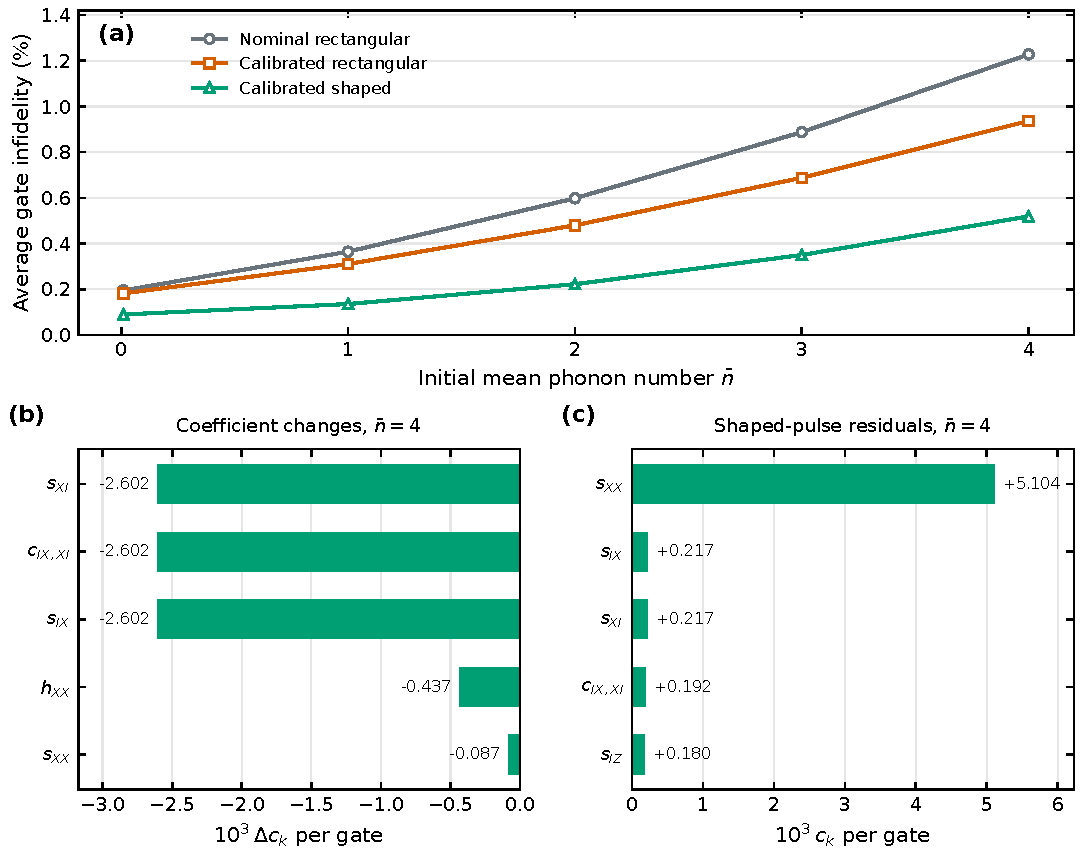
\includegraphics[width=\linewidth]
    {figures/pulse_shaping_residual_errors_100us.pdf}
    \caption{
        Suppression of residual errors by pulse shaping at
        \(T=100\,\mu\mathrm{s}\), with all four noise sources
        at their nominal rates.
        (a) Average gate infidelity for the nominal rectangular,
        calibrated rectangular, and calibrated shaped pulses.
        Markers indicate \(\bar n=0.01,1,2,3,4\); connecting
        lines are guides to the eye. Calibrated amplitudes are
        determined separately at each occupation.
        (b) The five largest absolute changes in generator
        coefficients at \(\bar n=4\), showing the signed differences
        \(\Delta c_k=c_k^{\mathrm{shaped}}-c_k^{\mathrm{rect}}\)
        between the two calibrated pulses.
        (c) The five largest residual coefficients of the calibrated
        shaped pulse at \(\bar n=4\), selected by absolute magnitude.
        Coefficient values in (b) and (c) are multiplied by \(10^3\).
        The comparison fixes gate duration but allows different peak
        drive amplitudes and keeps optical scattering rates fixed.
    }
    \label{fig:pulse_shaping_residual_errors}
\end{figure}

% Insert after the paragraph reporting the shaped-pulse diamond
% distance from nbar=0.01 to nbar=4, before the tolerance discussion.
\begin{figure}[htbp]
    \centering
    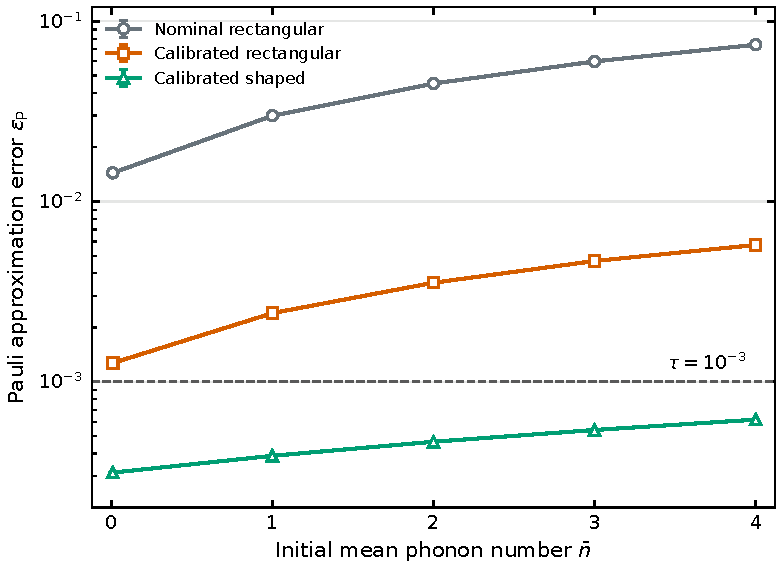
\includegraphics[width=0.88\linewidth]
    {figures/pauli_distance_three_conditions_100us.pdf}
    \caption{
        Pauli approximation error for the nominal rectangular,
        calibrated rectangular, and calibrated shaped pulses at
        \(T=100\,\mu\mathrm{s}\), with all four noise sources
        at their nominal rates.
        Each reconstructed error channel is compared with its own
        Pauli twirl using
        \(\epsilon_{\mathrm P}=\tfrac12
        \|\mathcal E-\mathcal E_{\mathrm P}\|_\diamond\).
        Calibrated amplitudes are determined separately at each
        initial occupation. The vertical axis is logarithmic.
        Markers indicate numerical estimates at
        \(\bar n=0.01,1,2,3,4\); connecting lines are guides to the eye.
        Error bars show numerical lower and upper bounds from the
        semidefinite programs and are smaller than the markers.
        These bounds do not include dynamical-simulation uncertainty.
        The dashed line indicates the illustrative tolerance
        \(\tau=10^{-3}\).
    }
    \label{fig:pauli_distance_pulse_shaping}
\end{figure}
